\documentclass[../main.tex]{subfiles}

\graphicspath{{\subfix{../images/}}}

\begin{document}

\section{Part 1 - Modelling and Simulations}

\subsection{Task 1.1}

Draw a complete equivalent circuit model of the buffer hip including all the signals of the drivers outputs, GDN and VCC supplies, the associated package parasitics for each of the paths and the PCB transmission lines including termination components.

\solution

We start by modelling the supply. The schematic is shown in Figure \ref{fig:supply} and component descriptions are summarized in Table \ref{tab:supply}.

\begin{figure}[h]
    \centering
    \fbox{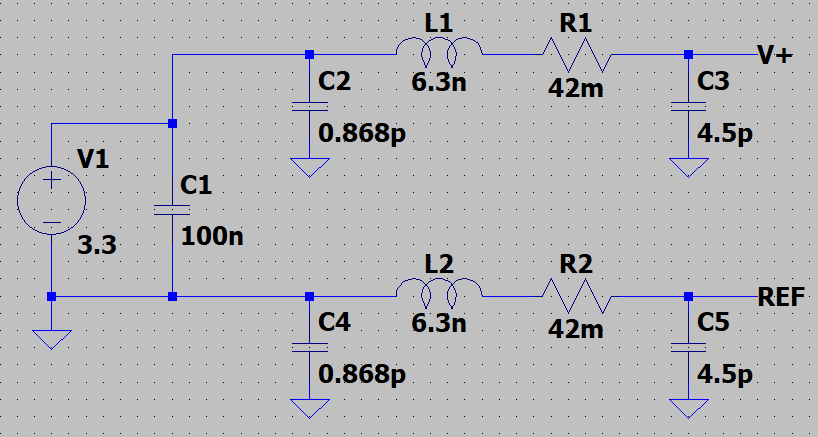
\includegraphics[width=0.8\textwidth]{supply.png}}
    \caption{LTSpice supply model.}
    \label{fig:supply}
\end{figure}

\begin{table}[h]
    \centering
    \begin{tabular}{l|r r}
        \toprule[1pt]
        \textbf{Component} & \textbf{Description} & \textbf{Source}\\
        \midrule
        $C_1$       & Supply decoupling & (Board schematic) \\
        $C_2/C_4$   & 74ALVC244 VCC pin capacitance & (IBIS) \\
        $L_1/L_2$   & 74ALVC244 VCC pin inductance & (IBIS) \\
        $R_1/R_2$   & 74ALVC244 VCC pin resistance & (IBIS) \\
        $C_3/C_5$   & 74ALVC244 input pin capacitance & (Datasheet) \\
        \bottomrule[1pt]
    \end{tabular}
    \caption{Supply model components descriptions.}
    \label{tab:supply}
\end{table}

Next we model the driver, receiver and transmission line inbetween. Shown in Figure \ref{fig:driver} and Table \ref{tab:driver}.

\begin{figure}[h]
    \centering
    \fbox{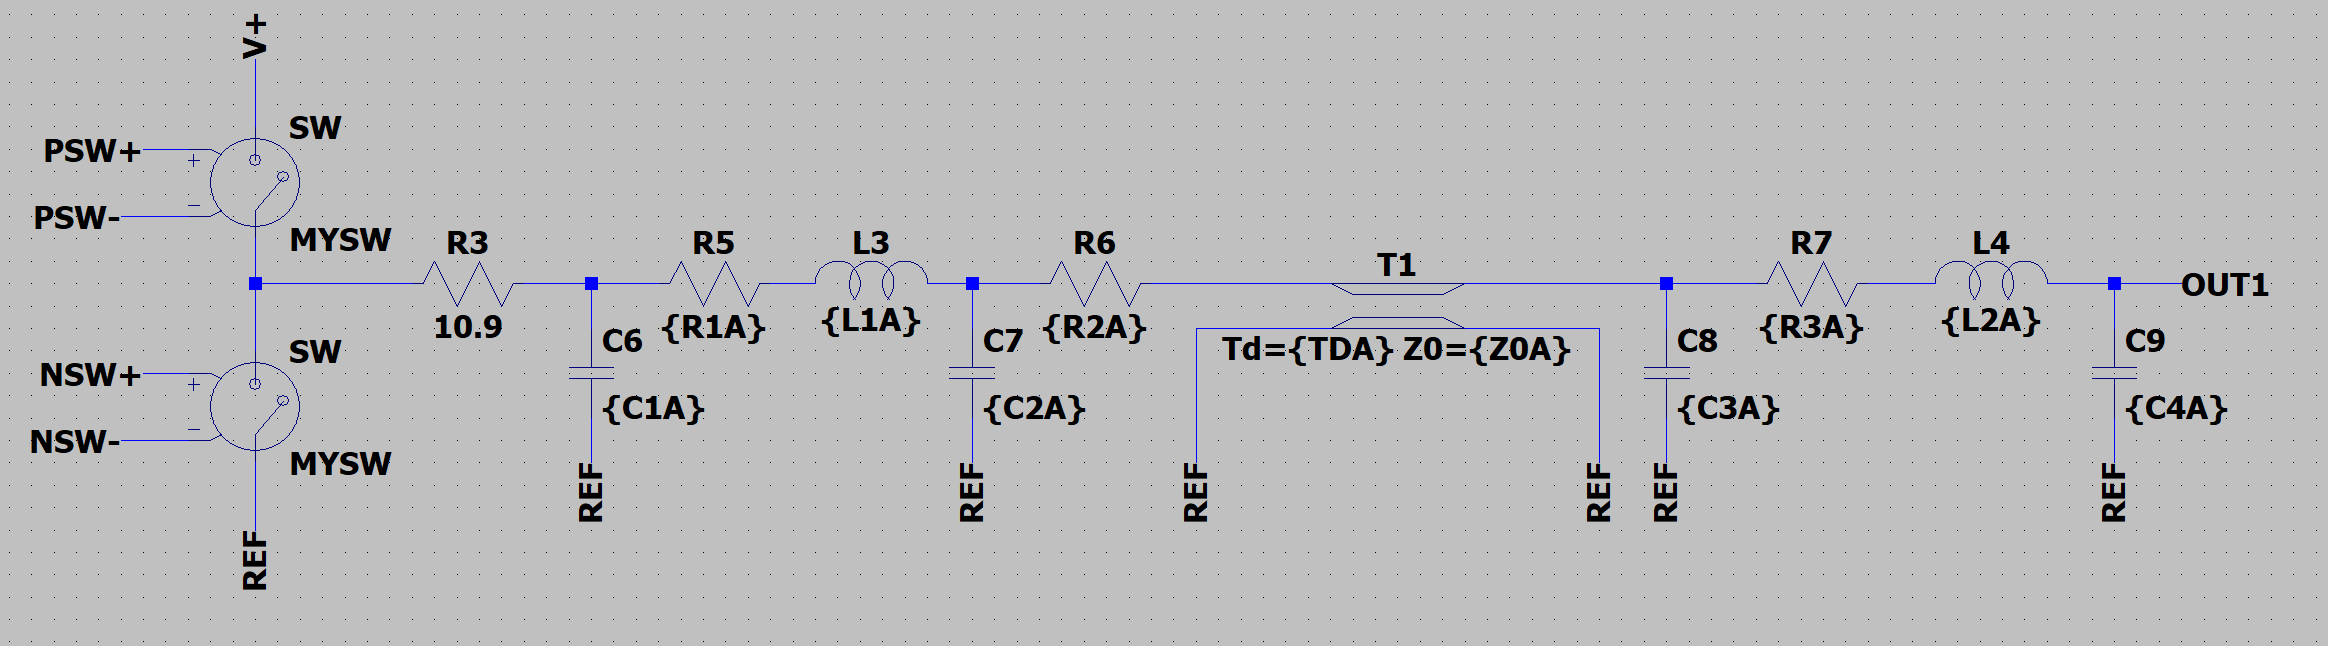
\includegraphics[width=0.9\textwidth]{ltspice_model.png}}
    \caption{LTSpice model of the system.}
    \label{fig:driver}
\end{figure}

\newpage

\begin{table}[h]
    \centering
    \begin{tabular}{r|r r}
        \toprule[1pt]
        \textbf{Component} & \textbf{Description} & \textbf{Source}\\
        \midrule
        $SW$    & CMOS totem pole output.       & \\
        $R_3$   & 74ALVC driver resistance      & \\
        $C_6$   & 74ALVC244 driver capacitance  & (IBIS) \\
        $R_5$   & Driver package resistance     & (IBIS) \\
        $L_3$   & Driver package inductance     & (IBIS) \\
        $C_7$   & Driver package capactiance    & (IBIS) \\
        $R_6$   & Board resistor                & (Board schematic)\\
        $T_1$   & PCB trace transmission line   & \\
        $C_8$   & Receiver package capacitance  & (IBIS) \\
        $R_7$   & Receiver package resistance   & (IBIS) \\
        $L_4$   & Receiver package inductance   & (IBIS) \\
        $C_9$   & Receiver input capactitance   & (IBIS) \\
        \bottomrule[1pt]
    \end{tabular}
    \caption{System model components descriptions.}
    \label{tab:driver}
\end{table}

\subsection{Task 1.2}

Determine from the IBIS model for the driver/receiver IC the inductances of the signal, GND and VCC pins for the QFN and SOIC packages.

\solution

The package parameters for both the QFN and SOIC packages are shown in Table \ref{tab:pkg-params}. The values are averages of all input/output pins. In addition the output capacitance of the driver is $C_{driver} = 6.03 \si{pF}$ and input capacitance of the receiver is $C_{receiver} = 4.21 \si{pF}$. The output resistance of the driver is $10.9\si{\Omega}$.

\begin{table}[h]
    \centering
    \begin{tabular}{r|r r r r}
        \toprule[1pt]
        \textbf{Package} & \textbf{Pin} & $R_{pkg}$ [$\si{\Omega}$] & $C_{pkg}$ [$\si{pF}$] & $L_{pkg}$ [$\si{nH}$] \\
        \midrule
        QFN  & In  & 0.097 & 0.139 & 1.415 \\
        QFN  & Out & 0.097 & 0.139 & 1.415 \\
        SOIC & In  & 0.038 & 0.717 & 5.012 \\
        SOIC & Out & 0.038 & 0.717 & 5.012 \\
        \bottomrule[1pt]
    \end{tabular}
    \caption{Average package parameters for the 74ALVC244 buffer outputs (QFN/SOIC).}
    \label{tab:pkg-params}
\end{table}



\end{document}
